\section{Security} Needles to say that the development process comes together with analyzing security vulnerabilities and implementing the solution to reduce them. My implementation contains two points where the setup plays a big role: the solution for storing sensitive data such as access and refresh tokens and the configuration of communication between the client and server sides.


\subsection{Tokens storage} Access and refresh tokens are both very sensitive pieces of data. In the case of successfully stealing the refresh token, an attacker will get long-term access to the application, or a short term in the case with the access token. That is why it is important to store these tokens as securely as it is possible.\\

\noindent \textbf{Most common attacks:} 

\begin{itemize}
    \item \emph{Cross-site scripting (XSS) attacks.} This is a type of attack where an attacker injects malicious scripts into a web page viewed by other users. It basically happens when an application trusts a user and the content, which can be inserted by them. 
    \item \emph{Cross-site request forgery (CSRF) attacks.} In general, this attack can be described as tricking a user into unintentionally performing some action. In this way, attackers just use the user's account to perform some harmful requests.
\end{itemize}


\noindent \textbf{Types of browser storages:} 

\begin{itemize}
    \item \emph{Local storage.} Local storage is web storage that allows the saving of key-value pairs of data. It provides the stored data persistence across the page reloading and can fit up to 5MB of data. Content from the local storage cannot be automatically sent and it makes it prone to CSRF attacks. However, it is not considered secure storage for keeping sensitive data due to the vulnerability to XSS attacks.
    \item \emph{Session storage} Session storage is client-base storage available by the browser which is very similar to the local storage. It has the same memory limit and vulnerabilities. But in addition to that it does not provide the persistence of data, which is a disadvantage to the user experience due to the need for repeated authentication.
    \item \emph{Cookies} Cookies are another way of storing data using a browser. Cookies can store much less data - up to 4KB, which might not always be enough for storing big tokens, but it is absolutely enough for my implementation. Cookies are vulnerable to both CSRF and XSS attacks, but with a proper configuration of secure attributes they are less vulnerable than local or session storage. Cookies can also be configured to be automatically sent with every HTTP request or some certain request.
\end{itemize}

\subsubsection*{Solution for the refresh token.} The perfect solution for storing sensitive data in a browser does not exist and in order to keep the data secure there should be also implemented other vulnerability-reducing features like input data validation, escaping and others. However, with the proper use of security attributes, cookies are much more likely to mitigate those attacks. Moreover, using cookies for storing tokens is recommended by the OWASP community due to their secure configuration options. \\
I have come to the solution of storing the refresh token, which is the most sensitive token requiring persistence across page reloads, in httpOnly cookies. HttpOnly cookies must be set on the server side as they are not accessible for JavaSccirpt. Therefore, I had to adjust the implementation of sending and receiving the refresh token in the authentication microservice from the body of requests to cookies. Figure 4.5 shows the configuration of security attributes for the refresh token cookie.\\

\begin{figure}[h]
\centering
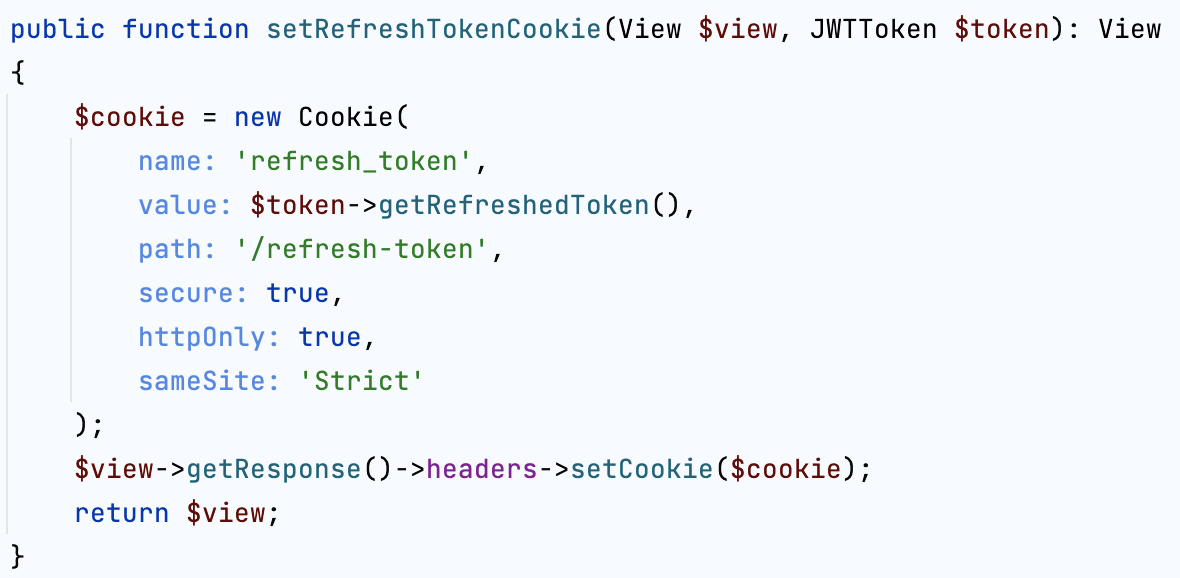
\includegraphics[scale=0.6]{../png/cookies.png}
\caption{Cookies setting}
\end{figure}

\noindent \textbf{Security attributes:}

\begin{itemize}
    \item \emph{Path.} URL path to which the cookie will be automatically sent.
    \item \emph{Secure.} This flag specifies that the cookie can be sent only through HTTPS ecrypted connections.
    \item \emph{HttpOnly.} The httpOnly flag is created to mitigate XSS attacks. With this flag, cookies can not be accessed by the Javascript.
    \item \emph{SameSite.} The strict value of that parameter means that the cookie is only sent if you are on the site that the cookie is set for. SameSite attribute is introduced for protection against CSRF. 
\end{itemize}


% https://www.invicti.com/learn/cookie-security-flags/

\subsubsection{Solution for the access token.} The access token is represented as JWT token, it contains the important information about the expiration time of the token and user's identity. It cannot be stored in the same way as refresh token as a client needs to have an access to that token directly.\\
Another way of storing the sensetive data which is considered more secure then local and session storages and cookies is storing it in memory(in a variable). This ways is considered more secure, because it is more prone to XSS attacks. The disadvantage of that method is that it doesn't provide the persistence, but in a case with access token it is a resolvable challenge.\\
First of all I have decided to store the access token and parsed information about user in the Pinia store, which is more secure then global variables.
%This store is shown in Figure 4.6.\\!!!

\begin{figure}[h]
\centering
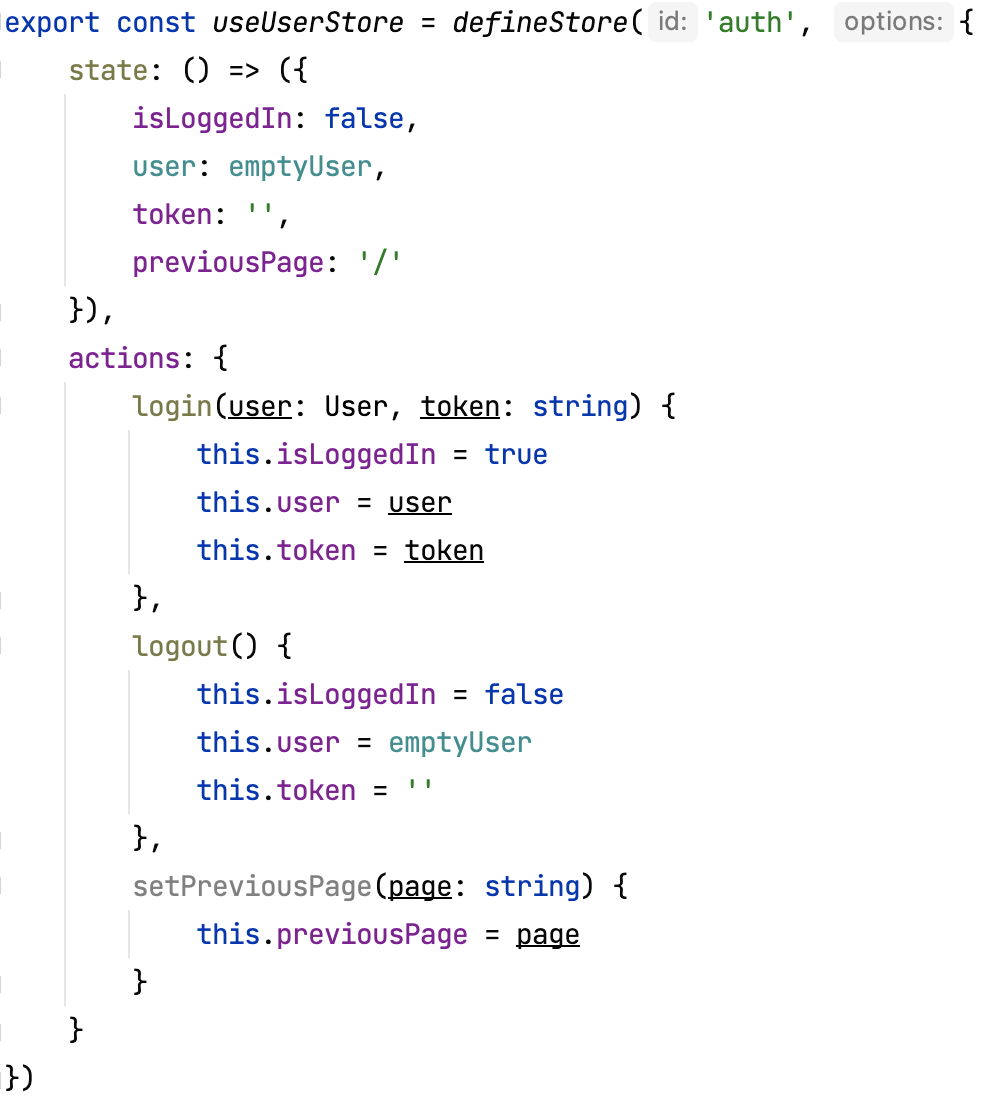
\includegraphics[scale=0.52]{../png/pinia_user.png}
\caption{Cookies setting}
\end{figure}

\noindent Pinia store is flexible and easy to use, that is an important moment because the stored information is used very often for sending requests, access control on the frontend and others.\\
Pinia storage does not provide data persistence on its own, but with the use of plugins it can enable this functionality with the use of local or session storage. Surely it is not suitable for the implementation as I am trying to use as most secure ways to store dat as it is possible. Therefore the users data will be lost together with an access token after the page reloads.\\
The BI-DBS is SPA application, meaning that page reloads are not a part of the usual functioning of the web page. However, for the case when a user does the page reload and store resets to the default values I have implemented the silent sign-in. Silent sign-in is shortened way of the authentication and authorization process described in 4.2.5. The user does not participate in this process, the client just quickly gets the access token as the authorization server already knows the user and does not require to provide the credentials before the access token expires.





\subsection{Communication with backend} Backend plays a huge role in the application and without it the frontend features I have implemented  would be non-functional. The backend and the frontend in the new BI-DBS portal are two separate units that communicate through HTTP requests. It is essential to correctly configure communication between them.

\subsubsection{Communication } Frontend sends HTTP requests to the backend using promised-based HTTP client Axios. Axios offers a wide range of configurations of the request. Starting from choosing a request type, setting an URL and body to interceptors for request and response. The example of configuring the Axios client is shown in Figure 4.7.

\subsubsection{HTTP headers} HTTP headers are vital components of communication between client and server. They provide detailed control over how requests and responses are managed, which leads improvements in such aspects as security, performance, and the user experience. Headers provide additional information about the HTTP request or response including security-related information like Cross-Origin Resource Sharing(CORS) and authorization. While access-allowance is set on the server side, the authorization is provided by the client. 

\paragraph*{Base configuration} For the base configuration of headers on the client side I have sent an accepted content type to application/json which can automatically be serialized and parsed to objects by Axios. The next header I have configured is the authorization header to contain the access bearer token. It is necessary for getting the data from a backend when it comes to different microservices from the authorization one. Other microservices require authentication and need to be provided with the access token in every request to validate the user and their access for making that request, which is implemented for security reasons. Header configuration is visualized in Figure 4.7.

\begin{figure}[h]
\centering
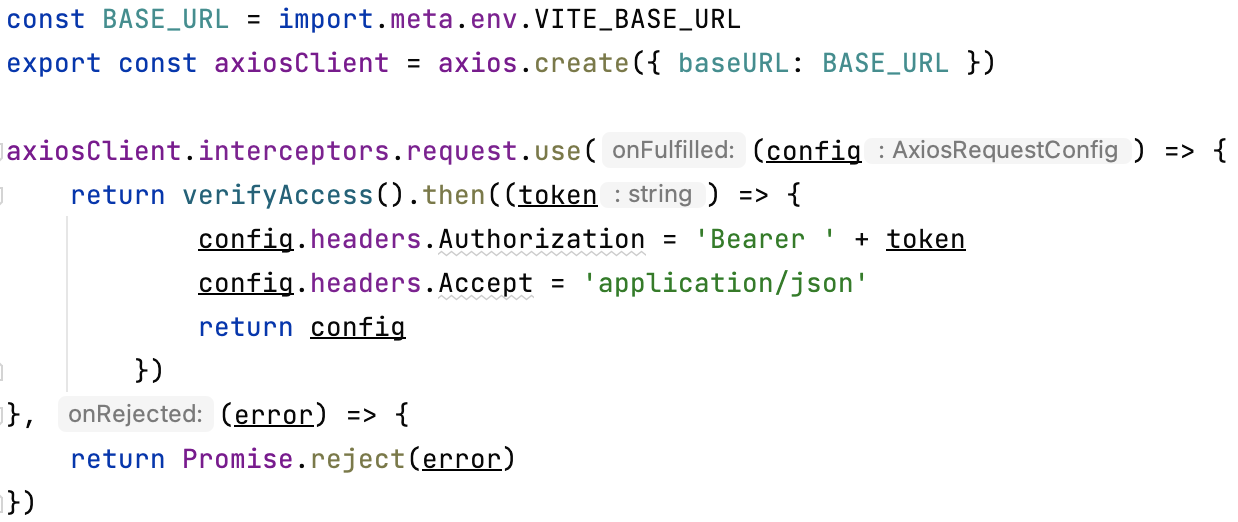
\includegraphics[scale=0.53]{../png/headers_base.png}
\caption{Axios base configuration}
\end{figure}


